\documentclass[report,gutter=10mm,fore-edge=10mm,uplatex,dvipdfmx]{jlreq}

\usepackage{lmodern}
\usepackage{amssymb,amsmath}
\usepackage{ifxetex,ifluatex}
\usepackage{actuarialsymbol}
\usepackage[]{natbib}
\RequirePackage{plautopatch}

% maru suji ① etc.
\usepackage{tikz}
\newcommand{\cir}[1]{\tikz[baseline]{%
\node[anchor=base, draw, circle, inner sep=0, minimum width=1.2em]{#1};}}

\usepackage{comment}

\begin{comment}

\ifnum0\ifxetex1\fi\ifluatex1\fi=0 % if pdftex
  \usepackage[T1]{fontenc}
  \usepackage[utf8]{inputenc}
  \usepackage{textcomp} % provide euro and other symbols
\else % if luatex or xetex
  \usepackage{unicode-math}
  \defaultfontfeatures{Scale=MatchLowercase}
  \defaultfontfeatures[\rmfamily]{Ligatures=TeX,Scale=1}
\fi
% Use upquote if available, for straight quotes in verbatim environments
\IfFileExists{upquote.sty}{\usepackage{upquote}}{}
\IfFileExists{microtype.sty}{% use microtype if available
  \usepackage[]{microtype}
  \UseMicrotypeSet[protrusion]{basicmath} % disable protrusion for tt fonts
}{}
\makeatletter
\@ifundefined{KOMAClassName}{% if non-KOMA class
  \IfFileExists{parskip.sty}{%
    \usepackage{parskip}
  }{% else
    \setlength{\parindent}{0pt}
    \setlength{\parskip}{6pt plus 2pt minus 1pt}}
}{% if KOMA class
  \KOMAoptions{parskip=half}}
\makeatother
\usepackage{xcolor}
\IfFileExists{xurl.sty}{\usepackage{xurl}}{} % add URL line breaks if available
\IfFileExists{bookmark.sty}{\usepackage{bookmark}}{\usepackage{hyperref}}
\hypersetup{
  hidelinks,
  pdfcreator={LaTeX via pandoc}}
\urlstyle{same} % disable monospaced font for URLs
\usepackage{longtable,booktabs}
% Correct order of tables after \paragraph or \subparagraph
\usepackage{etoolbox}
\makeatletter
\patchcmd\longtable{\par}{\if@noskipsec\mbox{}\fi\par}{}{}
\makeatother
% Allow footnotes in longtable head/foot
\IfFileExists{footnotehyper.sty}{\usepackage{footnotehyper}}{\usepackage{footnote}}

\end{comment}
%\makesavenoteenv{longtable}
\setlength{\emergencystretch}{3em} % prevent overfull lines
\providecommand{\tightlist}{%
  \setlength{\itemsep}{0pt}\setlength{\parskip}{0pt}}
\setcounter{secnumdepth}{-\maxdimen} % remove section numbering

\author{kazuyoshi}
\date{}

\newcommand{\problem}[1]{\subsubsection{#1}\setcounter{equation}{0}}
%\newcommand{\answer}[1]{\subsubsection{#1}}
\newcommand{\answer}[1]{\subsubsection{解答}}

%Pdf%\newcommand{\wakumaru}[1]{\framebox[3zw]{#1}}
\newcommand{\wakumaru}[1]{#1}






% \newcommand*{problem}[3]{\subsubsection{#1 生保#2 #3}}
% \newcommand*{answer}{\subsubsection{解答}}

\begin{document}
\section{保険1第7章 医療保険}
\section{7.1 民間医療保険の法的位置づけ}

\subsubsection{H24 生保1問題 1(3)
}
保険法に規定されている保険契約について、次の①~⑥の空欄に当てはまる適切な語句を答えなさ
い。
\begin{itemize}
 \item 生命保険契約とは、保険契約のうち、保険者が人の①又は②に関し一定の③を行うことを約するもの(傷害疾病定額保険契約に該当するものを除く。)をいう。
 \item 損害保険契約とは、保険契約のうち、保険者が一定の④
によって生ずることのある損害を⑤
することを約するものをいう。
 \item 傷害疾病定額保険契約とは、保険契約のうち、保険者が人の傷害疾病に基づき一定の
③を行うことを約するものをいう。
 \item 傷害疾病損害保険契約とは、⑥のうち、保険者が人の傷害疾病によって生ずることのある損
害(当該傷害疾病が生じた者が受けるものに限る。)を⑤することを約するものをいう。
\end{itemize}

\subsubsection{解答}

① 生存
② 死亡
③ 保険給付
④ 偶然の事故
⑤ てん補
⑥ 損害保険契約

\subsubsection{H9 生保1問題 1(1)}
保険業法第 3 条は生命保険会社および損害保険会社の事業に係わる免許について規定しているが、
以下の①~⑤のうち生命保険会社の事業に該当するものに○、該当しないものに×を付けよ。

\begin{itemize}
 \item [①] 人が疾病にかかったことを事由として一定額の保険金を支払う保険の引受け
 \item [②]
疾病にかかったことを原因とする人の状態を事由として生ずることのある当該人の損害をてん補する保険の引受け
 \item [③]
傷害を受けたことを直接の原因とする人の死亡に関して一定額の保険金を支払う保険の引受け
 \item [④]
傷害を受けたことを直接の原因とする人の死亡によって生ずることのある当該人の損害をてん補
する保険の引受け
 \item [⑤]
出産およびこれを原因とする人の状態に関して一定額の保険金を支払う保険の引受け
\end{itemize}

\subsubsection{解答}
①…・○、②…・○、③…・○、④…・○、⑤…・○

\subsubsection{H14 生保1問題 1(2)}
生命保険業免許は保険業法第 3 条第 4 項に規定されている。同規定に関して次の①~⑤を適当な語
句で埋めよ。

「生命保険業免許は、第一号に掲げる保険の引受けを行い、又はこれに併せて第二号若しくは第三号に
掲げる保険の引受けを行う事業に係る免許とする。

\begin{itemize}
 \item [一]  人の①
(当該人の余命が一定の期間以内であると医師により診断された身体の状態を含む。
以下この項及び次項において同じ。
)に関し、 ②
の保険金を支払うことを約し、保険料を収受
する保険(次号ハに掲げる死亡のみに係るものを除く。
)
 \item [二] 次に掲げる事由に関し、 ②
の保険金を支払うこと又はこれらによって生ずることのある当該
人の損害をてん補することを約し、保険料を収受する保険
\begin{itemize}
 \item [イ]
 人が疾病にかかったこと。
 \item [ロ]
③を受けたこと又は疾病にかかったことを原因とする人の状態
 \item [ハ]
③を受けたことを直接の原因とする人の死亡
 \item [ニ]
 イ又はロに掲げるものに類するものとして内閣府令で定めるもの(人の死亡を除く。)
 \item [ホ]
 イ、ロ又はニに掲げるものに関し、 ④ (
④
に類する行為として内閣府令で定めるもの
を含む。
)を受けたこと。
\end{itemize}
 \item [三]
 次項第一号に掲げる保険のうち、
⑤
であって、前二号に掲げる保険に係るもの」
\end{itemize}

\subsubsection{解答}
①生存又は死亡②一定額③傷害④治療⑤再保険

\subsubsection{H28 生保1問題 1(1)}
以下の保険業法および保険業法施行規則の抜粋について、次の①~⑤に適切な語句を記入しなさい。

【保険業法第3条(免許)】\\
【省略】\\

4.生命保険業免許は、第1号に掲げる保険の引受けを行い、又はこれに併せて第2号若しくは第3号
に掲げる保険の引受けを行う事業に係る免許とする。
\begin{itemize}
 \item [一]
人の①
(当該人の…【中略】…同じ。)に関し、一定額の保険金を支払うことを約し、保険
料を収受する保険(次項ハに…【中略】…を除く。)
 \item [二]
次に掲げる事由に関し、一定額の保険金を支払うこと又はこれらによって生ずることのある当
該人の損害をてん補することを約し、保険料を収受する保険
\begin{itemize}
 \item [イ]
 人が②にかかったこと。
 \item [ロ]
③を受けたこと又は②にかかったことを原因とする人の状態
 \item [ハ]
③を受けたことを直接の原因とする人の死亡
 \item [ニ]
 イ又はロに掲げるものに類するものとして内閣府令で定めるもの(人の死亡を除く。)
 \item [ホ]
 イ、ロ又はニに掲げるものに関し、治療(治療に類する…【中略】…を含む。)を受けたこと。
\end{itemize}
 \item [三] 次項第1号に掲げる保険のうち、再保険であって、前2号に掲げる保険に係るもの
\end{itemize}
【省略】\\
【保険業法施行規則第4条(②等に類する事由)】\\

法第3条第3項第2号二に規定する内閣府令で定める事由は、次に掲げる事由とする。
\begin{itemize}
 \item [一]
④及びこれを原因とする人の状態
 \item [二]⑤を要する身体の状態
 \item [三]老衰を直接の原因とする常時の介護を要する身体の状態
 \item [四]骨髄の提供及びこれを原因とする人の状態
\end{itemize}

\section{7.2 医療保険の商品傾向}
(過去問での出題はなし)
\section{7.3 医療保険の代表的保障内容}
\subsection{不担保期間、待期間、保険期間、給付限度}
\subsubsection{H13 生保1問題 1(10)、H1 生保1問題 1(5)}
医療保険の不担保期間を簡潔に説明せよ。
\subsubsection{解答}
・不担保期間
不担保期間には二つの考え方がある。「一定日数以上入院した場合、
入院日数に入院給付金日額を乗じて全額支払うが、一定日数以下の入
院に対しては給付しない方法」と「一定日数未満の入院に対して給付
金額を支払わないのは同じであるが、一定日数以上入院した場合は入
除日数から一定日数を差し壱1いた日数に入院給付金日額を乗じた金額
を支払う方法」である。不担保期間の設定により軽度の入院が抑制.さ
れ、国の医療費抑制政策とも合致する。
\subsubsection{H13 生保1問題 1(10)、H4 生保1問題 1(4)}
医療保険の待期間を簡潔に説明せよ。
\subsubsection{解答}
・待期間
責任開始期を契約日から一定期間遅らせる場合、その一定期間を
待期間という。故意入院または契約前発病を実務上効果的に排除し、
このような危険を回避する。しかし、待期間の制度は大多数の善意の
契約者に対しても、契約直後の入院に対して給付されないことになる
ので、商品設計の際には、契約者間の公平性の確保と契約者二一ズの
側面などからの検討を要する。
\subsubsection{H24 生保1問題 1(1)}
入院日数に応じて入院給付金を給付する医療保険
(1 入院の限度日数 30 日)
の開発を検討している。

1 ヶ月間の入院患者の在院期間別統計は次のとおりである。
次の(ア)、(イ)の各問に答えなさい。
\begin{tabular}[t]{|c|c|c|c|c|c|c|}
\hline 入院日数(日)& 1(日帰)& 2&3 & 4&5 &6--10 \\
 \hline 患者数(千人) &38.6 &123.1 &99.4 &64.8 &64.3 &289.0 \\ \hline
入院日数(日) & 11~15& 16~20& 21~25& 26~30&31~ & 総数\\ \hline
患者数(千人)
 & 148.7
& 89.9& 62.0& 44.1& 235.7& 1,259.6\\ \hline
\end{tabular}

統計調査時の被保険者対象範囲の人口は 127,962 千人とする。
\begin{itemize}
 \item [ (ア)]
 次の給付設計とした場合の粗の入院発生率と粗の給付日数を求めなさい。 なお、入院日数の階
 級値は中央値を採用することとする。
\begin{itemize}
 \item [○] 免責期間:3日
 \item [○] 免責方式:免責期間を超えた場合、全入院日数の保障を行う方式(フランチャイズ方式)
 \item [※]  入院発生率は年間の発生率をパーセント単位で答えること。また、答えはすべて小数点以下
 第2位を四捨五入して小数点以下第1位まで表すこと。
\end{itemize} 
 \item [(イ)]
 フランチャイズ方式を採用する場合において、一般的にリスク管理上留意すべき事項を簡潔
 に述べなさい。
\end{itemize}
\subsubsection{解答}
\begin{itemize}
 \item [(ア)]  粗発生率 9.4%[(64.8+64.3+…+235.7)÷127,962×12]\\
       粗給付日数 16.2 日[(64.8×4+64.3×5+…+235.7×30)÷(64.8+64.3+…+235.7)]
 \item [(イ)] フランチャイズ免責期間を長期間に設定すると免責日数を超過する日数で受取給付額が0
  から急激に増加するので意図して入院期間を延ばそうとする誘引が働き、モラルリスクの
 恐れが考えられる。日帰り入院を不担保とするなど、短期に設定するのが望ましく、長期
 の免責については免責期間の超過部分のみを保障する方式(エクセス方式)が適している。
\end{itemize}

\subsubsection{H20 生保1問題 4(2)①、H16 生保1問題 3(1)①、H7 生保1問題 1(1)} 
 医療保険の商品設計にあたり、リスク管理の観点からモラルリスクの回避等を目的として、保障内容
 に組み込む方策を簡潔に説明しなさい。
\subsubsection{解答}
\begin{itemize}
 \item [○] 待期間の設定:\\
 一定の範囲内で責任開始期を契約日から遅らせる場合のその期間のことをいう。
\begin{itemize}
 \item 被保険者があらかじめ疾病入院することが確実な場合、それを隠して契約に加入し、
 契約直後に疾病入院し、給付金を請求する場合がある。そのような悪意ある保険加入
 者を排除するための制度として待期間を設ける方法がある。
 \item この制度は免責期間とも言われ、がん保険などの場合に使用されることが多い。がん
 保険では告知の前または告知の時からがん給付の支払に関する責任開始のときまでに
 被保険者についての悪性新生物が診断確定された場合には、保険契約者および被保険
 者の、その事実の知・不知にかかわらず保険契約を無効とする約款規定がある。
 \item この制度を導入すると、善意の大多数の契約者に対しても、契約直後に給付がなされ
 ないため、この制度を設ける商品の選択は消費者の理解を得られるものに限るなど、
 慎重な判断が求められる。
\end{itemize}
 \item [○] 給付限度(日数限度)の設定:\\
 普通保険約款において設けられている給付日数の限度のことをいう。
\begin{itemize}
 \item これは二つの事柄から成り立っている。一つは1入院の給付限度を定めるもので、例
 えば60日、120日、180日などの限度設定である。もう一つは通算での限度を設定す
 るもので、700日や1000日などが一般的である。
 \item この日数の限度設定は一般的に行われており、モラルリスクの回避、集中リスクの回
 避などさまざまな理由付けがなされている。
 \item がん保険などでは通算限度を設けないものが大半であるなど、この日数制限について
 は、対象とする疾病の特性を勘案する必要がある。
\end{itemize}
 \item [○] 不担保期間の設定:\\
 入院開始から一定の期間を保障の対象としない場合、その期間のことをいう。
\begin{itemize}
 \item この場合、二つの考え方がある。一つは、一定日数以上入院した場合には入院全日数
 分の給付金を支払うが、それ以下の入院に対しては給付しないというもの。もう一つ
 は、一定日数以上入院した場合、入院日数からその一定日数を控除した日数分の給付
 金を支払うというものである。
 \item 以前は、特約方式の入院保障商品では、一定日数を控除するタイプのものがほとんど
 であったが、現在は不担保期間そのものを設定しないものも多く販売されている。
 \item また、給付日数の上限が一定限度に抑えられている商品があった場合、もとの給付が
 途切れるタイミングでその後の保障をリリーフすべく、不担保期間を非常に長く取る
 追加商品を販売することもある。
\end{itemize}
 \item [○] 保険期間の短期化:\\
 保障期間を短くし、長期保障から生じる不確実性のリスクを軽減することをいう。
\begin{itemize}
 \item 以前は、医療系商品または入院特約は一定期間を保障するもののみであったが、高齢
 化社会の到来により高齢期または終身まで保障する商品の二一ズが高まったこともあ
 り、現在は保険期間について、定期型商品と終身型商品が並立している。
 \item しかし、長期の医療保障、特に終身医療については将来的な基礎率の見込みが完全と
 は言えず、その都度におけるリスク・マネージメントが必要となる。そのようなリス
 ク対応の一環として別途、危険準備金の拡充による対応がなされている。
\end{itemize}
\end{itemize}
\subsection{トンチン}
\subsubsection{H13 生保1問題 2(1)①}
医療保険における死亡保険金(給付金)に関する「トンチン状態」を定義し、保険数理的な観点から
これが持つ問題点を記せ。
\subsubsection{解答}
\begin{itemize}
 \item  死亡保険金(給付金)(以下、死亡保険金)に関する「トンチン状態」の定義\\
 医療保険等では医療保障部分の発生率が高年齢ほど高くなり、加入年 齢・保険期間に
よっては医療保障部分の責任準備金が高額になることが ある。
医療保障要素を重視した商品で死亡保険金を小額に抑えている場
 合、保険期間の後半で責任準備金額が死亡保険金額を上回ることがある。
 このように保険期間中に責任準備金額が死亡保険金額を上回ることを
 死亡保険金に関する「トンチン状態」という。
 \item  トンチン状態から発生する問題点\\
 解約返戻金の水準を責任準備金に沿って定めている場合、トンチン状態
 では解約返戻金額が死亡保険金額を上回る場合が生じる。保険経営の健
 全性、保険契約者間の公平性を保険数理的に考慮すると次の事項などが
 問題点として挙げられる。
\begin{itemize}
 \item  死亡危険の近づいている契約者は、解約した方が受取額が大きいこと
 から解約の支払いを請求することとなり、死亡保険金を支払う以上に
 支払いが多くなる。このような支払いの増加は保険料計算上考慮され
 ていないため、収支の悪化を招くこととなり健全性が損なわれる。
 \item  解約返戻金額が死亡保険金(給付金)額を上回ることを知っているか
 どうかで受取額が異なることとなり、保険契約者間の公平性が保たれ
 ない。
 \item  保険契約を継続して死亡保険金を受け取る意味がなくなり、解約が促
 進されかねない。そして、保険料計算や責任準備金評価時に想定し許
 容していた以上に解約が起こると、当初の予測収益が得られなくなり、
 残存の保険群団の維持に支障をきたす恐れがある。
\end{itemize}
\end{itemize}

\subsubsection{H20 生保1問題 3(2)}
死亡保障が小額の医療保険(単品)を開発する場合、いわゆるトンチン性の問題から、解約返戻金額
が死亡保障の金額を超過する状態が発生する恐れがある。このような状態を回避するため、解約返戻金
および死亡保障の設計の側面から考えられる対応策を 3 つ挙げ、それぞれ簡潔に説明しなさい。
\subsubsection{解答}
\begin{enumerate}
 \item 約款の規定として解約返戻金額の上限を死亡保障の金額で抑えるが、保険料計算等に
は織り込まない方法
\begin{itemize}
 \item 保険料計算上、解約返戻金を死亡保障まで引き下げることについて考慮しない方法であ
るため、保険契約者から多めの保険料を恒常的に徴収することとなり、保険数理上は完
全な解決策とはならない。
 \item しかし、保険契約は約款規定に附合して成立するものであるため、保険契約者が約款規
定に合意した場合、契約そのものとしては問題がなく、また、通例、この引き下げ分を
保険料換算しても小額である場合も多いことから、契約者保護の観点からも問題ない場
合が多い。
\end{itemize}
 \item 予定解約率を用いて解約返戻金を死亡保障以下に設計する方法(例えば、解約返戻金
を死亡保険金額と同一とするなど、解約返戻金を「給付」として設計する方法)
\begin{itemize}
 \item 従来の、解約返戻金を責任準備金べ一スとする考え方では、保険料計算等は死亡脱退の
みを考慮して行うが、この方法の場合、予定解約率を用いることにより、死亡と解約の
2つの脱退事由を織り込んで保険料計算等を行うこととなる。
 \item 実際の解約が予定通りに発生して、収支が相当すれば問題ないが、予定解約率と実際の
解約率の相違により、収支のバランスが崩れる可能性がある。予定解約率をどのように
設定するか、また、解約率の変動に対してどのような対応を講ずるか等につき留意が必
要となる。
\end{itemize}
 \item 解約返戻金が死亡保険金額を超過する場合はその超過部分も死亡給付として支払い、
その分保険料に反映する方法(②とは逆に、解約返戻金を制限するのではなく、死亡
保障を解約返戻金の水準まで引き上げる方法)
\begin{itemize}
 \item 死亡保障の引き上げ分は、解約返戻金と契約上の死亡保険金額の差額に死亡率を乗じ、
現価計算することにより、保険料計算等に反映されるため、その分、②に比べ保険料は
高くなる。
 \item 理論上は引き上げた死亡給付からも責任準備金・解約返戻金が生じるが、実務上はこれ
以上の高階の責任準備金計算はしない近似的な方法となり、完全な解決策とはならない。
 \item また、医療単品において技術的な理由から死亡保障を引き上げることについて商品性と
してどこまで妥当であるか等の問題も残る。
\end{itemize}
\end{enumerate}
\subsubsection{H22 生保1問題 2(2)}
平準払の生命保険商品(第三分野商品を含む。)の商品設計上責任準備金が負値となることが発生ず
る場合がある。どのような場合に負値責任準備金が発生しうるか例示を交えて説明し、負値責任準備金
の発生がもたらす問題点を述べ、商品を開発するにあたり留意すべき事項を簡潔に述べなさい。ただ
し、ここで扱う負値責任準備金は平準純保険料式で算出されるものに限る。
\subsubsection{解答}
負値責任準備金は主に平準払の定期保険で、
\begin{itemize}
 \item [①]発生率(死亡率)が年齢とともに逓減する場合
 \item [②]給付金額(保険金額)が年齢あるいは経過年数とともに逓減する場合
\end{itemize}
などの理由により危険保険料が年数の経過につれて減少する場合において発生しうる。
通常は各年齢における危険保険料は年齢が高くなるにつれて上昇するので、年齢が若い間に平準払保
険料の一部を将来の危険保険料の上昇に対する備えとして保険料積立金として積み立てることとなる
のでこのような負値責任準備金が発生することはない。ところが各年齢における危険保険料が年齢の高
まりにつれて減少する場合はこの関係が逆転し、年齢が若い間の危険保険料の一部を将来の平準払保険
料から賄う形となり、責任準備金は負値となる。
計算処理上は負値の責任準備金は0として処理されることが一般的である。そのため、責任準備金が
負値となる状態で解約が生じた場合に不足分を契約者から徴求できないにもかかわらず、収入保険料が
不足した状態で契約が消滅するため、保険契約全体での収支バランスが悪化することが想定される。ま
た、契約時年齢が高まるにつれて平準私営業保険料が逓減することも考えられ、その場合責任準備金が
負値となる間に解約し改めて新しい契約年齢において加入しなおした方が保険料を安くできるケース
が想定され、中途解約の増加、未解約の契約者との間の公平性の欠落などの問題が発生し得る。
このような点を踏まえて、「保険会社向けの総合的な監督指針」においては、給付が逓減する場合や
保険料を後払いする場合においては責任準備金が負値とならないように設定することとされており、計
算上負値の責任準備金を0とする場合は財務の健全性に関する十分な検討がなされていることに留意
することが求められている。
負値の責任準備金を回避するには、
\begin{itemize}
 \item [①]発生率について適切なスムージング等を行い、年数の経過によって逓減しないようにする
 \item [②]負値の責任準備金が生ずる契約パターンを販売できないようにする
 \item [③]負値責任準備金が生じない他の給付(保障)と組み合わせる
\end{itemize}
などの対応が考えられる。①の場合においては保険料の適正性や契約者問の公平性に問題がないか
配慮する必要があり、②の場合は過度に契約者に理解し難い形態とならないよう配慮しつつ販売形態
を構築する必要があるといえる。
\subsubsection{H23 生保1問題 2(3)}
保険種類の中には、保険期間中に「責任準備金額>死亡保険金(給付金)額」という状態が発生する
ことがある。
\begin{itemize}
 \item [①] このような状態が起きる例を 2 つ挙げよ。
 \item [②] 責任準備金額に応じて単純に解約返戻金額を定めた場合、
「解約返戻金額>死亡保険金(給付金)
額」となる場合がある。このような解約を認める場合の問題点を簡潔に述べよ。
 \item [③] ②の状態を防ぐための方法を 3 つ挙げ、それぞれの方法の留意点も含めて説明せよ。
\end{itemize}
\subsubsection{解答}
\begin{itemize}
 \item [①] 以下のような例から2つを回答する。
\begin{itemize}
 \item 年金保険やこども保険のように生存保障要素を重視する保険
 \item 死亡に至る前の被保険者生存中の医療保障要素を重視する一方で死亡保険金(給付金)額
を小さくしている(場合によってはOとしている)保険
 \item 一定期間経過後、死亡保険金額がアップする、あるいは死亡保険金額が逓増するタイプの保険
\end{itemize}
 \item [②]死亡保険金より解約返戻金の受取額が大きい場合、契約を継続して死亡保険金を受け取る意
味がなくなり、特に健康状態の悪化した場合などに解約が促進され、保険料計算時に想定し
ていた死亡が発生しない等、「保険契約群団の維持」に支障をきたす恐れがある。
さらに、死亡直前に解約を行って解約返戻金を受け取った場合と解約せずに死亡保険金で受
け取った場合とでは、解約の方が受取額が大きくなるので、公平性の観点から問題が生ずる
恐れがある。
 \item  [③] ②の状態を防ぐための方法として例えば次の3点が挙げられる。
\begin{itemize}
 \item 該当するケースが発生するような場合は規定等で取扱範囲を制限する。\\
この方法は抜本的な対策ではなく、ごく一部分で生じる場合に緊急避難的に該当ケース
を除外するものであるが、契約締結可能範囲のほとんど全てで生じる場合には、商品の売
り止めや商品改訂が必要となる。
 \item 解約返戻金を死亡保険金(給付金)額以下に強制的に抑える。\\
保険料計算に解約率を織り込んでいない場合は、解約返戻金の水準引下げが保険料の引
下げに貢献せず、解約した際の当該部分の解約益は、過去の事業費支出の精算とは無関係
なものとなる。この解約益は、将来生じるかもしれない群団としてのコストを残存契約群
団だけではなく、脱退契約群団にも負担してもらうという考え方に基づいて精算されるも
のと考えられる。
 \item 解約自体を制限する。\\
年金保険の終身年金開始後で使用されることが多い。この取扱に関しては、契約者の解
約権を阻害していることにならないかという問題がある。契約者の任意解約権に関しては、
約款上承認された約定解約権という理解が一般的であるため、約款に規定した上で契約が
成立している以上問題ないと考えられる。
\end{itemize}
 \item [【別解】]以下は第7章r医療保険」に掲載されている事項。
\begin{itemize}
 \item 予定解約率を用いて解約返戻金をデザインする。\\
例えば、予定解約率を用いて解約返戻金を死亡保険金と同一とし、死亡保険金と同一の
額を解約のときに「給付」する。この場合、予定解約率を適正な水準に見込んでおく必要
があり・その見積もりいかんでは大きな収支損が発生する可能性がある。
 \item 解約返戻金部分を死亡給付の一部とする。\\
解約返戻金が死亡保険金額を超過した場合は超過した部分も死亡給付として支払う方法
で、この部分も保険料に反映させる。正確には解約返戻金と死亡保険金額の差額部分に対
して生じる責任準備金額も手当てしなければならないので、完全にこの方法で問題を解決
することは困難で、あくまで近似的な方法に過ぎないことに留意しなければならない。
\end{itemize}
\end{itemize}
\section{7.4 医療保険の保険料計算}
\subsection{医療保険の予定発生率の設定}
\subsubsection{2021 生保1問題 3(1)①, H27 生保1問題 3(2)①}
医療保険の開発時において、予定発生率作成に用いる基礎データとして、自社データを用いる場合と
公共データを用いる場合がある。それぞれのメリット・デメリットを簡潔に説明しなさい。(4点)
\subsubsection{解答}
\begin{itemize}
 \item 自社データのメリット(○)、デメリット(×)
\begin{itemize}
 \item ○過去にも同様の保障内容の商品を販売していた場合、自社の査定方法、選択効果、販売チャネル等、個社の状況に基づいた分析を行うことができる。
 \item ○公共データに比べて、男女別・年齢別・経過別など詳細なデータを取得できる場合が多い。
 \item ×一般的に公共データよりデータ量(母数)が少なく、分析に十分な信頼性が得られない可能性が
ある。特に定常状態の集団になっていない場合、そのまま用いると過小評価となる。
 \item ×過去に類似の商品がない場合は、自社データの使用は困難である。
 \item ×基礎データへ逆選択(モラルリスク)の影響が生じる可能性がある。
\end{itemize}
 \item 公共データの(○)、デメリット(×)
\begin{itemize}
 \item ○データ量(母数)が多い。基礎データへの逆選択(モラルリスク)の影響は小さいと考えられる。
 \item ○過去未販売の新たな支払事由等、自社データに比べて、幅広いデータを取得できる。
 \item ×開発する商品の支払事由に完全に適合するデータがない場合があり、使用目的に沿った(何らかの)補整が必要となる。
 \item ×選択効果の反映、また自社独自の査定を行っている場合はそれを反映するかどうかを別途検討す
る必要がある。
\end{itemize}
\end{itemize}

\subsubsection{H20 生保1問題 4(2)②、H16 生保1問題 3(1)②、H15 生保1問題 3(1)、H10 生保1問題 2(1)①、H7 生保1問題 1(1)、H2 生保1問題 2(2)、}
医療保険の予定発生率等の設定が、死亡保険の予定死亡率の設定に比べて考慮を要する理由を挙げ、
それぞれ簡潔に説明しなさい。
\subsubsection{解答}
\begin{itemize}
 \item ○医療保険の有する危険性がより主観的である。
\begin{itemize}
 \item 障害状態の存在や医的治療の必要性は、死亡の事実ほど早期には確定しない。また、
災害死亡給付については、その死亡が事故を原因とするか否かも判定しなければなら
ない。このように、医療保険の場合、給付にあたっての事実認定に主観的要素が混入
しやすいことが挙げられる。
 \item また、契約の更新等においては、健康でない人がより継続するという(所謂リスク濃縮)
問題もあり、これも主観的な行動が伴うため、対応した予定発生率等の予測が難しい。
\end{itemize}
 \item ○医療保険の経験値には、死亡保険の経験値が有する危険性とは本質的に異なる次の要
素がある。
\begin{enumerate}
 \item 経済・社会動向に対してより顕著に反応すること
 \item 医療技術の変化、医療費水準の高度化および医療機関の利便性の拡大によって影響
を受けること
\end{enumerate}
\begin{itemize}
 \item 経済・社会動向の場合、例えば、平均在院日数はベッド数が人口に比して少ない時期
または地域では、短期のものにシフトすることになる。
 \item 医療技術の場合、例えば、胃切除術の後に以前は1ヵ月程度入院していた者が今では
2週間程度で済むようになった結果、ベッドの占有期間が短縮されることなどである。
\end{itemize}
 \item ○死亡に比べて統計データが不十分である。
\begin{itemize}
 \item 医療保険の給付には様々な種類があるため、全ての給付に対し十分な量のデータを蓄
積することは困難である。これとともに、医療保険の経験値も日を追って変化するた
め、予定発生率等を算出するのに十分なデータを得ることが困難なものとなっている。
 \item 基礎的経験率は、これまでの経済・社会動向を反映したものであることを考慮して、
注意深く評価されなければならない。さらに、募集形態の多様化(ダイレクトメール
やインターネット等を利用した募集等販売チャネル)により、募集形態の差異が基礎
的経験率へ影響するかどうかも考慮する必要がある。
\end{itemize}
\end{itemize}
\subsubsection{H28 生保1問題 2(2)}
ある疾病に関する入院を保障する医療保険の開発において、公的データより粗発生率を作成したと
ころ、粗発生率は年齢に関し単調増加とならず、30 歳台に一部粗発生率が減少する年齢層があった。
この保険の予定発生率および営業保険料の設定について、以下の設問に答えなさい。

①粗発生率の形状をそのまま予定発生率に使用した場合の問題点について述べなさい。

②①の問題点への対応策を挙げ、これらを適用する際に留意すべき事項を述べなさい。
\subsubsection{解答}
①粗発生率の形状をそのまま予定発生率に使用した場合の問題点
\begin{itemize}
 \item 保険期間と保険料の逆転\\
年齢に関して単調増加でない粗発生率に対し、その形状を補正しないまま予定発生率を作成
する場合、有期保障については保険期間が長いほど保険料が安くなることが考えられ、その場
合、契約者が自分の入りたい保険期間より長い保険期間のなかでの最安値を選べば無リスクで
保険料を安くするオプションが存在するといった問題が生じる。
 \item 加入年齢と保険料の逆転\\
同様に、予定発生率の形状によっては年齢が高齢であるほうが保険料は安くなることが考え
られ、その場合、新しい契約年齢において加入しなおしたほうが保険料は安くなるため、中途
解約の増加や未解約の契約者との公平性の問題が生じる。
 \item 負値責任準備金の発生\\
責任準備金が負値となる状態で解約が生じた場合に不足分を契約者から徴求できないにも
関わらず、収入保険料が不足した状態で契約が消滅するため、保険契約全体での収支バランス
が悪化することが想定される。
\end{itemize}

② ①への対応策および留意すべき事項
\begin{itemize}
 \item 加入年齢と保険料の逆転といった上記問題点を許容する。\\
許容する場合、上記問題点で述べた解約の増加等による収益(財務の健全性)への影響や、負
値責任準備金の発生する範囲が限定的であることの確認が必要となる。また、特に保険期間と
保険料の逆転が生ずるケースでは、販売上(顧客説明)の観点からも問題点はないか確認する
必要がある。
 \item 許容しない場合は、以下の対応策等が考えられる。
\begin{itemize}
 \item [ア].発生率について適切なスムージング等を行い、年齢に関して単調増加となるよう補正する。\\
粗発生率の山について、当初の発生率を引き下げて補正を行う場合、保険料の十分性、
収益性の観点から問題がないか、収益検証などを実施し十分留意していく必要がある。ま
た、発生率を引き上げて補正を行う場合、契約者間の公平性の観点に留意する必要がある。
 \item [イ].営業保険料の計算の際に保険期間の長短比較を行い、保険期間と保険料の逆転が生じない
ようにする。\\
営業保険料の長短比較(付加保険料による調整)等により、保険期間と保険料の逆転が
生じないようにすることが考えられるが、保険料の引下げに相当する対応であり、保険料
の十分性、収益性の観点から問題がないか留意する必要がある。
 \item [ウ].販売範囲等(加入年齢や保険期間)を限定する。\\
一部の年齢範囲や保険期間について取扱を限定する場合、契約者(+募集者)からの理
解が得られるものであるか、顧客ニーズに合ったものとなっているかといった観点に留意
する必要がある。
 \item [エ].他の給付(保障)と組み合わせる。\\
結果として保険料が高くなってしまうため、顧客ニーズに合ったものとなっているかと
いった観点に留意する必要がある。
\end{itemize}
\end{itemize}
\subsubsection{2019 生保1問題 3(1)①}
給付事由が社会保険制度に連動する第三分野商品の予定発生率の設定は、死亡保険の予定死亡率の
設定よりも困難であることが想定される。以下の 2 つの点から、その理由を簡潔に説明しなさい。
\begin{itemize}
 \item 第三分野商品の予定発生率と死亡保険の予定死亡率を比較した場合の論点
 \item 給付事由が社会保険制度に連動する場合の論点
\end{itemize}
\subsubsection{解答}
\begin{itemize}
 \item 第三分野商品の予定発生率と死亡保険の予定死亡率を比較した場合の論点
\begin{itemize}
 \item 医療保険の有する危険性は、死亡に比べて発生がより主観的である(障害状態の存在や治療の必
要性は、死亡の事実ほど明確には確定しない。災害死亡給付については、その死亡が本当に事故を原因とするものか否かも判定しなければならない。)。
 \item 医療保険の経験率には、死亡保険の経験率が有するものとは本質的に異なる要素がある(経済・社会動向に対してより顕著に反応、医療技術の変化等によって影響を受ける)。
 \item 統計データが不十分(長期の観察を要する、同じ名称の統計データでも中身が変わっている場合もある)。
\end{itemize}
 \item 給付事由が社会保険制度に連動する場合の論点
\begin{itemize}
 \item 制度自体が大幅に変更になることがある。
 \item 制度自体は維持されながら、活用している定義の詳細が変わる。
\end{itemize}
\end{itemize}
\section{7.5 医療保険の責任準備金等}
\subsection{医療保険の事業年度末責任準備金}


\subsubsection{H5 生保1問題 1(1)改}
医療保険の事業年度末責任準備金を簡潔に説明せよ。
いわゆる入院責任準備金、IBNR 備金および両者の関係
\subsubsection{解答}

\paragraph{医療保険の事業年度末責任準備金は次の二つの部分の合計額として評価する。}

\begin{itemize}
 \item 未経過保険料\\
一つは通常の死亡保険と同様に、対象契約を契約年度毎に分け、同一契約年度の契約
は年央で契約したものとみなして、年度始と年度末の保険年度末責任準備金の和半
によって求める翌事業年度以降発生分の給付の現価、
 \item いわゆる入院責任準備金\\
もう一つは当該事業年度中に
入院が発生していながら、事業年度末では入院継続中により給付金請求が行われず、
翌年度以降に請求される給付金のための責任準備金として評価するもので、
$$\xi_{x+t-1}\cdot T_{x+t-1}\cdot\frac{T_{x+t-1}+N}{365}$$
によって求める。通常の責任準備金の補正項である。

$\xi_{x+t-1}$: 第t保険年度の入院発生率\\
$T_{x+t-1}$: 第t保険年度の平均在院日数\\
$N$:不担保期間
\end{itemize}

\paragraph{保険業法施行規則(第72、73条)で積立を要求される支払備金}

支払備金:当該事業年度中に入院が発生し支払い義務が発生したが、何らかの理由で事業年度末に当該事由に対する支払がなされていない場合等の積立金(負債の部;未払金,経常費用;支払備金等繰入額)で、以下の2種類がある. 

\begin{enumerate}
\item 支払義務が発生しているが、決算期において、まだ支出として計上して
いない保険金等
\item 払事由の発生の報告を受けていないが、支払事由が既に発生したと認め
られる保険金等(いわゆる「IBNR(既発生未報告)備金」)
\end{enumerate}

\paragraph{いわゆる入院責任準備金、IBNR 備金および両者の関係}

いわゆる入院責任準備金の対象となる請求は
決算期にはまだ入院が継続している状態を表している。

既発生未報告支払備金の対象である請求は
事業年度内に退院の時期を迎えている
(すなわち、支払事由があり、その支払事由が確定している)が、
いわゆる入院責任準備金の対
象となる請求は決算期にはまだ入院が継続している状態を表している。
次の
図はこの二つの関係を示したものである。
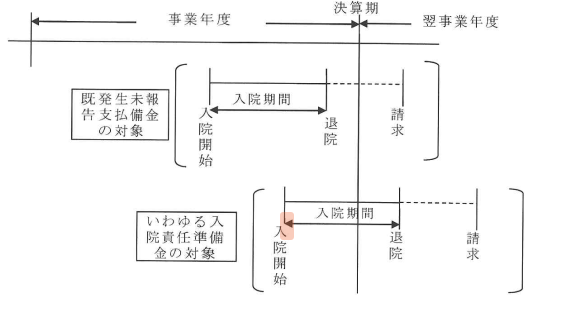
\includegraphics[scale=0.8]{images/ProbH5-1-1-1.png}

ただし、これは、「いわゆる入院責任準備金」が通常の責任準備金の補正項である、という立場を崩したものではない。

\subsubsection{H17 生保1問題 1(4)}
入院したときに、入院給付金として「給付金日額×入院日数」を支払う医療保険がある。この医療保
険の責任準備金に関する以下の設問に解答せよ。

入院給付部分の責任準備金には、評価日時点で入院中であり評価日時点以降に請求金額が確定する部
分に対する責任準備金(入院継続中部分の責任準備金)があるが、給付金日額 1 あたりの入院継続中部
分の責任準備金を、予定入院発生率ξおよび予定給付日数丁を使って表記し、かつ、なぜそう記述でき
るのかを説明せよ。ただし、不担保期間は無く、1 年間の日数は 365 日、ξおよび T は被保険者の年齢
や経過によらず一定値とする。
\subsubsection{解答}
年間での入院発生率はξ、給付対象となる入院の平均日数はTであることから、評価
日時点において入院が継続中である確率は、$\xi \frac{T}{365}$ となる。
また、一入院に対しての予定給付額は、給付金日額1あたり、給付金日額(=1)×予定
給付日数(=T)=Tとなる。
したがって、入院継続中部分の責任準備金は、予定給付金日額×評価日時点において
入院継続中である確率と書き表すことが出来るので、
$\xi T\frac{T}{365}$ となる。
\subsubsection{H2 生保1問題 1(5)}
医療保険の IBNR 備金を簡潔に説明せよ。
\subsubsection{解答}
支払備金計上方法は、保険業法施行規則第28条に規定されているが、同条は
「既発生既報告で未払のものを計上する。」と解釈され、既発生未報告(IBNR)備金は、日本では計上されていない。
しかし、医療保険においては、入院給付金は退院後に請求されることが多く、
保有契約の増加により既発生未報告分は無視し得なくなってきている。
なお、事業年度末に入院継続中と予定されるものについては、
責任準備金に計上されており、IBNR備金には含まれない。

\subsubsection{H28 生保2問題 1(5)、H25 生保1問題 1(6)}
医療保険の入院給付について、既発生未報告支払備金といわゆる入院責任準備金の概要、および両
者の関係を簡潔に説明しなさい。
\subsubsection{解答}

責任準備金の一部として、いわゆる入院責任準備金の積み立てが行われており、「支払事由は発
生しているがその請求金額の確定がいまだなされていない」状態を扱っているものである。
責任準備金の補正的項目として、事業年度をまたぐ入院給付の蓋然性を計算する。
既発生未報告支払備金の対象である請求が、事業年度内に退院の時期を迎えているが報告を受
けていない状態であるのに対して、いわゆる入院責任準備金の対象となる請求は、決算期にま
だ入院が継続している状態である。

---
\begin{itemize}
 \item 既発生未報告支払備金は、保険会社が、決算期において、まだ支払事由の発生の報告を受けて
いないが、保険契約に規定する支払事由が既に発生したと認める給付について、その支払いに
必要な金額である。支払備金の一部として積み立てる。
 \item いわゆる入院責任準備金は事業年度をまたぐ入院給付の蓋然性を計算し、それを責任準備金の
一端として計上するもの。
 \item 既発生未報告支払備金の対象である請求は事業年度内に退院の時期を迎えており支払事由が確
定しているのに対して、いわゆる入院責任準備金の対象となる請求は事業年度末時点ではまだ
入院が継続しているという違いがある。
\end{itemize}


\subsection{第三分野ストレステストと負債十分性テスト}
\subsubsection{H23 生保2問題 1(1)}
第三分野保険のストレステストに関し、以下の①~⑤の空欄に当てはまる適切な語句または数字
を記入しなさい。
\begin{itemize}
 \item テスト実施期間(10 年間以上)について、
「保険事故発生率に対するリスクの①%をカバーする水準(X)」、
「保険事故発生率に対するリスクの 99%をカバーする水準(Y)」を予測し、
「②に基づく保険金額(Z)」と比較する。
 \item X,Y,Z の大小関係に応じて次のとおり危険準備金を積み立てる。
\begin{tabular}[b]{lcl}
 Z≧Y&⇒ & 保険料積立金が十分と判断する。\\
 Y>Z≧X& ⇒&保険料積立金が不十分として、「③」を危険準備金として積み立てる。\\
Y>X>Z &⇒&保険料積立金が不十分として、「④」を危険準備金として積み立てたうえで、保険料積立金が不足する恐れがあると判断し、⑤を実施する。\\
\end{tabular}
\end{itemize}
\subsubsection{解答}
①97.7
②予定発生率
③Y−Z
④Y−X
⑤負債十分性テスト
\subsubsection{H27 生保2問題 1(1)}
第三分野の責任準備金積立ルール・事後検証等に関する次の①~⑦の文章について、下線部分が正し
い場合は○を、誤っている場合は×を記入するとともに、誤っている場合は下線部分を正しい内容に改
めなさい。
\begin{itemize}
 \item [①] ストレステストのテスト実施期間は\underline{5}年間である。
 \item [②] ストレステストでは、発生率に関するリスクの \underline{99.5\%}をカバーする発生率を予測し、将来発生する
保険金額と、予定発生率に基づく保険金額を比較して、予定発生率に基づく保険金額が、将来発生
する保険金額を下回っていれば、保険料積立金が不十分として危険準備金を積み立てる。
 \item [③] ストレステストの保険事故発生率の将来予測において、どのようなモデルを設定するかは、\underline{保険会社}が合理的に見込む。
 \item [④] ストレステストの結果、予め設定した予定事故発生率では、保険料積立金で対応すべき「通常の予
測の範囲内のリスク」に対応できないおそれがある場合は、\underline{資産十分性テスト}による事後検証を行う。
 \item [⑤] ソルベンシー・マージン基準における第三分野保険の保険リスク相当額の計算において、「ストレ
ステストの対象とするリスク」のリスク対象金額は危険準備金積立限度額、リスク係数は \underline{0.5} である。
 \item [⑥] 医療、がん、介護等の区分ごと\underline{危険保険料}に対する保険金等の支出の状況を開示する。
 \item [⑦] 商品認可申請時等において、第三分野保険の保険契約に関する保険料及び責任準備金の算出方法書
の記載事項が保険数理に基づき合理的かつ妥当なものであることについて、\underline{保険会社}が確認した結果を記載した意見書を申請書に添付する。

\end{itemize}
\subsubsection{解答}

\begin{tabular}{|c|c|c|}
 ①&× & 10 \\
 ②&×& 99\\
 ③&◯& \\
 ④&×& 負債十分性テスト\\
 ⑤&× & 1/10 \\
 ⑥&× & 保険料 \\
 ⑦&× & 保険計理人 \\
\end{tabular}

\subsubsection{H29 生保2問題 2(1)、H19 生保2問題 2(4)}
第三分野保険のストレステストおよび負債十分性テストについて、導入された背景およびそれぞれ
の概要を簡潔に説明しなさい。
\subsubsection{解答}
\paragraph{(導入された背景)}
\begin{itemize}
 \item 少子高齢化社会が進行するなかで、医療や介護といったいわゆる第三分野保険商品のニーズが高
まっている。これらの商品は、医療政策等の外的要因や契約者の想定外の行動の影響を受けやす
く、また日本では終身保障タイプの商品が多いこと等から長期にわたりリスクを負うこととなる。
 \item 第三分野保険商品は、商品内容が多種多様であり、十分なデータの蓄積もないことからスタンダ
ードな指標が存在しておらず、公的なデータや各社の実績等から給付事由ごとに発生率を見込ま
ざるを得ない状況となっている。
 \item このようなことから、保険会社において適切なリスク管理が行われ、将来の債務履行のために必
要な水準の責任準備金の積立が可能となるよう、事後的にモニタリングや保険料積立金・危険準
備金の十分性の検証等を行っていくこととなった。
\end{itemize}
\paragraph{(ストレステスト)}
\begin{itemize}
 \item 毎決算期に、商品ごとにあらかじめ設定した予定事故発生率が十分なリスクをカバーしているか
を確認するために実施する。
 \item テスト実施期間(10年間以上)について、「通常の予測を超える範囲でリスクをカバー(保険
事故発生率に対するリスクの99%をカバー)する水準の将来給付額(A)」、「通常の予測の範
囲でリスクをカバー(保険事故発生率に対するリスクの97.7%をカバー)する水準の将来給
付額(B)」を予測し、「予定発生率に基づく将来給付額(P)」と比較する。
 \item A、B、Pの大小関係に応じて次のとおり危険準備金を積み立てる。
\begin{tabular}{lcl}
P≧A&⇒&保険料積立金が十分と判断する。\\
A>P≧B &⇒&保険料積立金が不十分として、「A-P」を危険準備金に積み立てる。\\
B>P&⇒&保険料積立金が不十分として、「A-B」を危険準備金に積み立てたうえで、
保険料積立金が不足する恐れがあると判断し、負債十分性テストを実施する。\\
\end{tabular}
 \item 第三分野保険商品の保障内容やリスクの範囲は多岐にわたっており、商品により異なることから、
保険事故発生率の将来予測におけるモデルは、保険会社が合理的に見込む。
 \item 「保険期間が1年以下の保険契約(更新時に保険料率が変更可能なもの)
」、
「傷害保険契約その他
これに準ずる給付を行う保険契約」、
「保険事故発生率が十分小さい、特約又は主たる給付に付随
する給付であり、債務の履行に支障を来たすおそれが極めて低い保険給付」はストレステストの
対象外とする。
\end{itemize}
\paragraph{(負債十分性テスト)}
\begin{itemize}
 \item ストレステストの結果、予め設定した予定発生率では、保険料積立金で対応すべき「通常の予測
の範囲内のリスク(リスクの97.7%)」に対応できない恐れがある場合は、負債十分性テス
トによる事後検証を実施する。
 \item 保険料積立金の十分性については、収入支出全体の動向を踏まえ、実質的な不足が生じているか
を判断する必要があるため、将来収支分析により検証を行う。
 \item 実績等をもとに将来の収入・支出を推計し、資産が負債である保険料積立金を下回ることがない
か確認する(テスト実施期間:10年以上)。
 \item 資産=保険料積立金としてスタートする。
 \item 将来時点の資産は、実績等から推計した各年の収入・支出をもとに計算する。なお、この際に用いる保険事故発生率は、危険発生率(保険事故発生率が変動することによる保険金の増加を97.7%の確率でカバーする保険事故発生率)を用いる。
 \item 将来時点の保険料積立金は予定基礎率をもとに計算する。
 \item 上記をもとに、テスト期間中の事業年度末における資産と保険料積立金の比較を実施する。資産
が保険料積立金を下回った場合は積立不足と判断し、不足額(保険料積立金-資産)の割引現在
価値の最大値を追加して責任準備金を積み立てる必要があることを、保険計理人の意見書に記載
しなければならない。
\end{itemize}

\subsubsection{2022 生保1問題 1(3)}
第三分野保険に関する次の①~④について、下線
部が正しい場合は「正」と記入し、誤って
いる場合は正しい表現に改めなさい。(4点)
\begin{enumerate}
 \item [①] 第三分野商品の\underline{販売開始}時には、保険数理に基づき合理的かつ妥当であることについて、保険計
 理人が確認した結果を記載した意見書を金融庁に提出することが保険業法施行規則において求め
 られている。
 \item [②] 第三分野保険のストレステストでは、実績の保険事故発生率等に基づいてテスト実施期間の発生
 率に関するリスクの \underline{97.7%}をカバーする発生率を予測し、将来発生する保険金額と予定発生率に基
 づく保険金額を比較して、保険料積立金の十分性を判定する。
 \item [③] 保険会社向けの総合的な監督指針によると、第三分野保険の\underline{ストレステスト}において、新契約の
 募集を停止し、かつ被保険者数が少なくなったことにより、大数の法則が機能せず、結果として収
 支相等の原則の適用が困難なときは、当該契約集団の給付額を支出見込額として使用することがで
 きるとしている。
 \item [④] 入院給付金の\underline{IBNR備金}の対象となる請求は、決算期にまだ入院が継続している状態である。
\end{enumerate}
\subsubsection{解答}
① 認可申請 ② 99% ③ 負債十分性テスト ④ (いわゆる)入院責任準備金


\section{7.6 基礎率変更権の取扱}
\subsection{2020 生保1問題 1(6)}
第三分野保険の基礎率変更権について、次の①、②の各問に答えなさい。
\begin{enumerate}
 \item [①]  保険業法施行規則第 11 条第1項第7号イにおける「第三分野保険の基礎率変更権」の定義を簡
 潔に説明しなさい。(1点)
 \item [②] 保険会社向けの総合的な監督指針(Ⅳ-4-1 基礎率変更権の設定について)に規定されてい
 る3つの「基礎率変更権行使基準の設定にあたって満たすべき要件」および「整備することが必要
 となる態勢」について簡潔に説明しなさい。(4点)
\end{enumerate}
\subsubsection{解答}
\begin{itemize}
 \item [①] 実績発生率が予測と相違する(ことが見込まれる)ため、予定発生率を変更して保険料また
 は保険金を変更する権利。
 \item [②] 基礎率変更権行使基準の設定にあたって満たすべき要件 :
\begin{enumerate}
 \item [( 1)] 予定発生率に対する実績発生率の状況を示す指標が「予定発生率に対する実績発生率の割
 合」または「保険料収入に対する保険金の支出額の割合」
 (に準じたもの)となっている
 こと。
 \item  [(2)]指標が、実績発生率が悪化した場合の損益見込みに照らして、適切な水準となっているこ
 と。
 \item  [(3)]指標に達した後、保険料または保険金の変更を行う手続きが、明確になっていること。
\end{enumerate} 
 \item 整備することが必要となる態勢 :\\
 実績発生率の管理や基礎率変更権の行使の意思決定を行う態勢。
\end{itemize}
\subsection{H26 生保1問題 1(6)、H21 生保1問題 2(1)}

保険会社向けの総合的な監督指針における第三分野保険の基礎率変更権の設定について、以下の問
に答えなさい。
\begin{itemize}
 \item [①]基礎率変更権行使基準の設定にあたっての満たすべき要件を挙げなさい。
 \item [②]基礎率変更権の行使のための認可申請があった場合の審査の際の留意点を 4 つ挙げなさい。
\end{itemize}

\subsubsection{解答}

\begin{itemize}
 \item [①]基礎率変更権行使基準の設定にあたっての満たすべき要件
\begin{enumerate}
 \item [1)]予定発生率に対する実績発生率の状況を示す指標については、予定発生率を変
更して保険料又は保険金を変更するという趣旨に適合するものとして、次に掲げ
るいずれかの割合又は当該割合に準じたものとなっているか。
\begin{itemize}
 \item [ア.]予定発生率に対する実績発生率の割合
 \item [イ.]保険料収入(責任準備金繰入・戻入調整をした当該年度の危険保険料と付加
保険料の合計)に対する保険金の支出額の割合
\end{itemize}
 \item [2)]1)に掲げる指標の設定にあたっては、実績発生率が悪化した場合の、当該保
険契約の損益見込みに照らして、適切な水準となっているか。
 \item [3)]1)に掲げる指標に達した後、保険料又は保険金の変更を行う手続きが、明確
になっているか。
\end{enumerate}
 \item [②]基礎率変更権の行使のための認可申請があった場合の審査の際の留意点
\begin{enumerate}
 \item 約款に定める基礎率変更権の規定(基礎率変更権行使基準等)に反しないものとなっているか。
 \item 社内において定められている基礎率変更権の行使の手続きが遵守されているか。
 \item  契約者に対して、契約締結時にあらかじめ十分な説明が行われ、その後も基礎率変更権行使基
 準に該当するかどうかの情報開示が定期的に行われていたか。
 \item  変更後の予定発生率が、実績発生率等に照らして保険数理に基づく合理的かつ妥当なものとな
っているか。
\end{enumerate}
\end{itemize}

\section{付録1 既発生未報告支払備金の評価方法}
\subsubsection{H14 生保1問題 1(4)}
入院給付に関する IBNR 備金について、次の問題に答えよ。\\
$X$を退院時から入院給付金請求時までの期間を表わす確率変数とし、その分布関数(退院時点から$t$
年以内に入院給付金請求がなされる確率)を$F(t)$とする。また、$t\geq 1$ のとき
$F(t)=1$と仮定する。
1 事業年度において、年始を$t=0$、年末を$t=1$とし、$S_t$ を時点$t$において会社が保有する入院給付金日額の総額とする。
入院給付金日額は各契約均一とする。1 入院の入院期間は一律$T$日、入院給付日数は入院の初日から
勘定するものとし、1 入院による給付金額は「$T$×入院給付金日額」とする。
また、ξを入院発生率とし入院は年間を通じて一様に発生するものとする。
このとき、以下の条件のもとで事業年度末($t=1$)における入院給付金の IBNR 備金の値を計算せよ。
なお、解答は百円単位を四捨五入して千円単位で求め、その計算過程についても記載すること。
〔条件〕
\begin{itemize}
 \item $\xi=0.01$
 \item $S_t=S_0\times(1+0.1\times t)$、ただし、$S_0=1$億円
 \item $T=20$日
 \item $X$ の平均値を m=0.1 (年)
 \item $X$ の標準偏差をσ=0.1 (年)
\end{itemize}
なお、1 年間の日数は 365 日とし、$\int_{0}^{1}F(x)dx = 1-m$, $\int_{0}^{1}x\cdot F(x)dx = \frac{1}{2}-\frac{1}{2}(m^2+\sigma^2)$
であることは断りなく使用してよい。
\subsubsection{解答}
IBNR備金の値 2169千円

[計算過程]\\
$[t, t+dt]$
で入院を開始した者に対する入院給付金総額は、$S_t\cdot T\cdot\xi\cdot dt$
である。
$t$で入院開始した者は年単位では
$t+T/365$で退院する。従って、$[t,t+dt]$で入院して年度末に未報告になっている金額は、
$S_t\cdot\xi\cdot T\{1-F(1-t-\frac{T}{365})\}dt$ である。

ここで、$T'=\frac{T}{365}$とおくと、\\
IBNR備金 = $\int_{-T'}^{1-T'}S_t\cdot\xi\cdot T\{1-F(1-t-T')\}dt$となる。\\
ここで, 仮定の$S_t=S_0\times(1+0.1\times t)$
を代入し, さらに,  $1-t-T'=x$と変数変換すると,\\
IBNR備金 = $\int_{0}^{1}\{S_0+(1-x-T')\times 0.1\times S_0\}\cdot\xi\cdot T\{1-F(x)\}dt$\\
$=\xi TS_0\{(1.1-0.1T')\cdot m-0.05(m^2+\sigma^2)\}$\\
これに所与の定数を代入すると、2,169,041円、従って、解答は2,169千円である。

\section{その他}
\subsection{H26 生保1問題 3(2)①}
医療保険の開発にあたり、商品設計、予定発生率の設定等に関し、一般的に留意すべき事項について
説明しなさい
\subsubsection{解答}
\begin{itemize}
 \item 医療保険の一般的な特徴
\begin{itemize}
 \item 医療保険は、多種多様な保障内容が提供されており、保険期間が終身にわたる商品も多い。
 \item 医療保険は、逆選択やモラルリスクを誘発する可能性が高いことや、医療技術の進歩等の外的要因
の影響を受けやすいといった、死亡保険と異なる危険性を有している。
 \item 商品設計・基礎率の設定にあたっては、こうした危険性への留意・工夫が必要。
\end{itemize}
 \item 商品設計上、一般的に留意すべき事項
\begin{itemize}
 \item 不担保期間、待期間、給付限度の設定
 \item 死亡給付や複数の給付、反対給付の組み込み
 \item 保険期間を短期とし、更新型とする
 \item 有配当とする(発生率の不確実性のリスクを軽減)
 \item 基礎率変更条項を約款上規定する(但し、契約者への情報提供等が必要となる)
\end{itemize}
 \item 予定発生率の設定に関し一般的に留意すべき事項
\begin{itemize}
 \item 
・医療保険の予定発生率等は、予定死亡率と比べ、次の理由により設定が困難である。設定にあたっ
てはその影響について留意する必要がある。
\begin{itemize}
 \item 医療保険の危険性は死亡に比べてより主観的。
 \item  医療保険の経験率には死亡保険とは異なる次の要素がある。
\begin{itemize}
 \item A.経済・社会動向に対してより顕著に反応する
 \item B.医療技術の変化等により影響を受ける
\end{itemize}
 \item  統計データが十分ではない場合がある。
\end{itemize}
 \item  なお、保険会社向けの総合的な監督指針では、予定発生率に関しては基礎データに基づいた合理的
な算出が求められている。
\end{itemize}
 \item その他留意すべき事項
\begin{itemize} 
 \item 将来的な基礎率の不確実性への対応の一環として、第三分野のストレステストや負債十分性テスト が導入されている。
 \item  解約返戻金ありの商品の場合、解約返戻金が死亡時の給付金を上回る、いわゆるトンチン性の問題 がある。
 \item  トンチン性の解消、保険料の低廉化を目的として、解約返戻金をなくした商品も多い。その場合、
 予定解約率の設定、実際の解約の変動が収支に及ぼす影響にも留意が必要。
\end{itemize}
\end{itemize}

\subsection{H27 生保1問題 3(2)②}
医療保険の商品販売開始後のフォローアップの必要性について、簡潔に説明しなさい。(4点)

\subsubsection{解答}
\begin{itemize}
 \item  近年、保険商品には、社会の構造的変化・経済活動の多様化等に伴い、国民の生活保障ニーズの
		     高まり、新たなリスクの発生など、保険契約者ニーズに対応すべく多様化が求められている。
 \item  こうしたニーズに応え、保険会社が商品開発を行うにあたっては、保険業法等の法令等を踏まえ、
  自己責任原則に基づき、リスク面、財務面、募集面、法制面等あらゆる観点から検討する内部管
  理態勢の整備が求められる。
\item 監督指針上においても、商品開発プロセスの中に商品販売開始後のフォローアップを組み込むこ
  とが明記されており、適切にフォローアップを行う体制を整備する必要がある。
\item 特に医療系商品についてはモラルリスクが混入しやすいことや経済・社会動向の影響を受けやす
  いことなど、死亡保障とは異なる特性を有している。また保障内容も多様化していることから、
  これまで引き受けた経験のないリスクを引き受ける必要が生じており、適切な予定発生率の検証
  等を行う必要性は高いと考えられる。
\item また、法令・監督指針において、第三分野ストレステスト・負債十分性テストを行うこととなっ
 ており、この観点からも第三分野商品の発生率の事後検証が重視されている。
\end{itemize}

\end{document} 